\documentclass{article}

\usepackage{graphicx}
\usepackage{tikz}
\usepackage{tikzsymbols}
\usetikzlibrary{calc,patterns,shapes.geometric}
\pagestyle{empty}
\usepackage[margin=0pt]{geometry}
\geometry{papersize={14in,12in}}

\def\centerarc[#1](#2)(#3:#4:#5){\draw[#1] ($(#2)+({#5*cos(#3)},{#5*sin(#3)})$) arc (#3:#4:#5);}

\begin{document}
	\begin{figure}
		\centering
		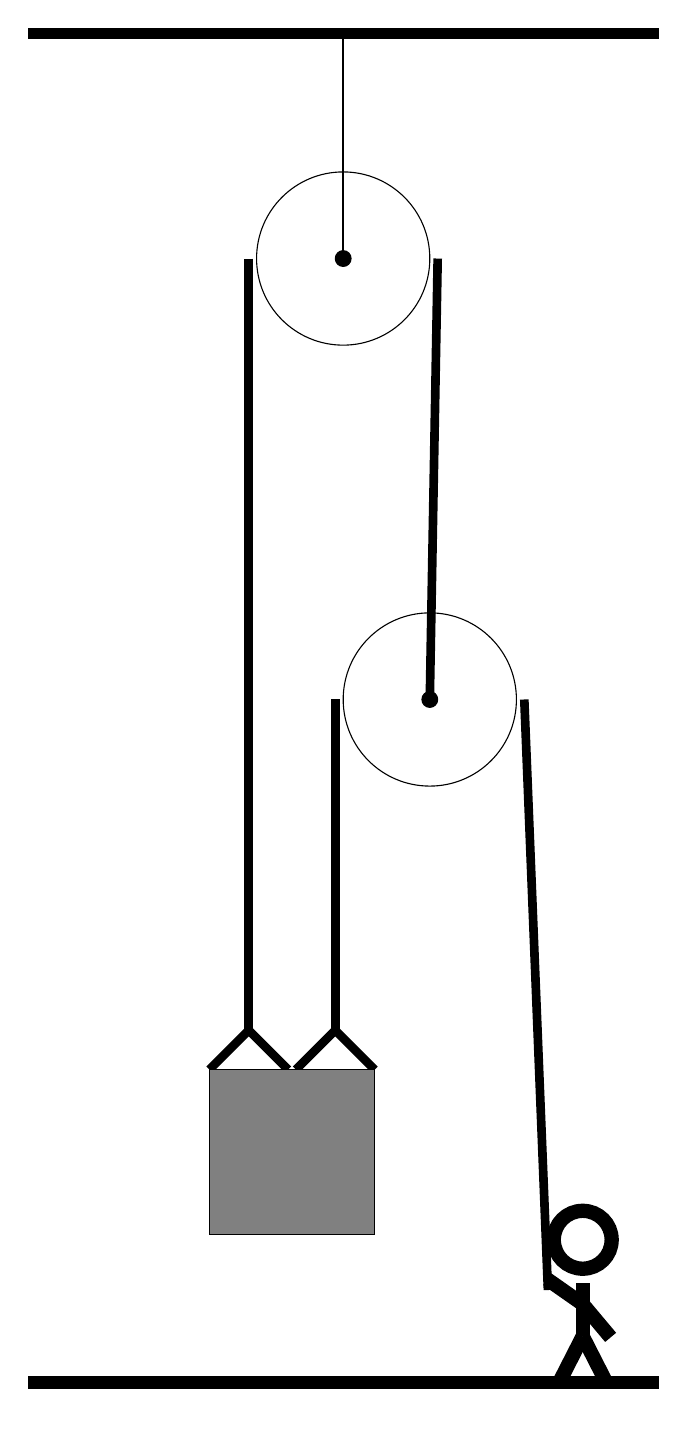
\begin{tikzpicture}
			%%%%% START %%%%%
			\draw[fill=black] (-2, 14) rectangle (6, 14.125);
			
			\draw (2, 11.2) circle (1.1);
			\draw[fill=black] (2, 11.2) circle (0.1);
			\draw[thick] (2, 11.2) -- (2, 14);
			
			\draw (3.1, 5.6) circle (1.1);
			\draw[fill=black] (3.1, 5.6) circle (0.1);
			
			\draw[line width = 1.1mm]  (0.3, 0.9) -- (0.8, 1.4) -- (1.3, 0.9);
			\draw[line width = 1.1mm]  (1.4, 0.9) -- (1.9, 1.4) -- (2.4, 0.9);
			\draw[fill=black!50] (0.3, 0.9) rectangle (2.4, -1.2);
			
			\draw[line width = 1.1mm] (0.8, 11.2) -- (0.8, 1.4);
			\centerarc[line width = 1.1mm](2, 11.2)(0:180:1.2000000000000002);
			\draw[line width = 1.1mm] (3.2, 11.2) -- (3.1, 5.6);
			\draw[line width = 1.1mm] (1.9, 5.6) -- (1.9, 1.4);
			\centerarc[line width = 1.1mm](3.1, 5.6)(0:180:1.2000000000000002);
			\draw[line width = 1.1mm] (4.3, 5.6) -- (4.6, -1.9);
			
			\node at (5, -2) {\Strichmaxerl[10][-35][-50]};
			
			\draw[fill=black] (-2, -3) rectangle (6, -3.15);
			%%%%% END %%%%%
		\end{tikzpicture}
	\end{figure}	
\end{document}